\appendix
\section{其余记录}
\label{sec:appendix}

表~\ref{tab:coverfull} 和表~\ref{tab:swapfull} 补上正文消融的六项绝对分。覆盖变体关闭问题交换。交换上限加在格子配额上，四档按记录中的递增顺序排列，正文不把具体次数写入方法。

\begin{table}[h]
\centering
\scriptsize
\setlength{\tabcolsep}{2.6pt}
\caption{覆盖补选的六项对照。MME 为感知分。}
\label{tab:coverfull}
\begin{tabular}{@{}lrrrrrr r@{}}
\hline
策略 & GQA & POPE & MME & MMB & SQA & Text & Rel.6 \\
\hline
旧覆盖 & 55.57 & 82.21 & 1339.28 & 61.34 & 68.91 & 53.41 & 93.47 \\
修空格与负余弦 & 55.96 & 81.50 & 1349.46 & 61.17 & 68.86 & 53.41 & 93.50 \\
空格去掉显著性 & 54.15 & 76.33 & 1298.96 & 59.45 & 69.26 & 52.93 & 90.96 \\
逐步更新原型 & 55.70 & 82.12 & 1371.95 & 60.14 & 69.51 & 53.73 & 93.77 \\
格子配额 & 55.92 & 81.48 & 1376.34 & 60.57 & 69.46 & 53.85 & 93.89 \\
残差放到锚点外 & 55.40 & 81.07 & 1363.77 & 60.14 & 68.86 & 53.82 & 93.27 \\
\hline
\end{tabular}
\end{table}

\begin{table}[h]
\centering
\scriptsize
\setlength{\tabcolsep}{2.6pt}
\caption{格子配额上的四档交换。MME 为感知分。}
\label{tab:swapfull}
\begin{tabular}{@{}lrrrrrr r@{}}
\hline
上限 & GQA & POPE & MME & MMB & SQA & Text & Rel.6 \\
\hline
关 & 55.92 & 81.48 & 1376.34 & 60.57 & 69.46 & 53.85 & 93.89 \\
最小一档 & 57.08 & 86.19 & 1408.92 & 61.51 & 69.86 & 53.28 & 95.66 \\
第二档 & 57.04 & 87.08 & 1395.42 & 60.65 & 68.62 & 52.00 & 94.78 \\
第三档 & 56.57 & 87.03 & 1356.98 & 59.79 & 67.82 & 51.54 & 93.68 \\
第四档 & 56.60 & 87.29 & 1327.41 & 58.85 & 67.67 & 51.16 & 93.02 \\
\hline
\end{tabular}
\end{table}

同一个 $W{=}1024$ 的三次首次收缩，保留序列与维持层数是 $(64,17,10)$ 对 $(12,8,12)$、$(128,24,16)$ 对 $(4,8,20)$、$(160,28,8)$ 对 $(4,8,20)$。三者同时改变入口和各档长度。历史中间档的四项绝对分是：中间 61 且维持很长，GQA 56.10、POPE 78.11、MME 总分 1720.1、MMBench 61.86；中间 90，57.18、82.99、1765.2、62.20；中间 148 但很快进入最终档，56.60、83.38、1781.6、59.88。末段“32 然后 12”与“24 然后 16”的六项均值是 96.78\% 与 96.89\%，MME 用感知分。

\begin{figure}[h]
\centering
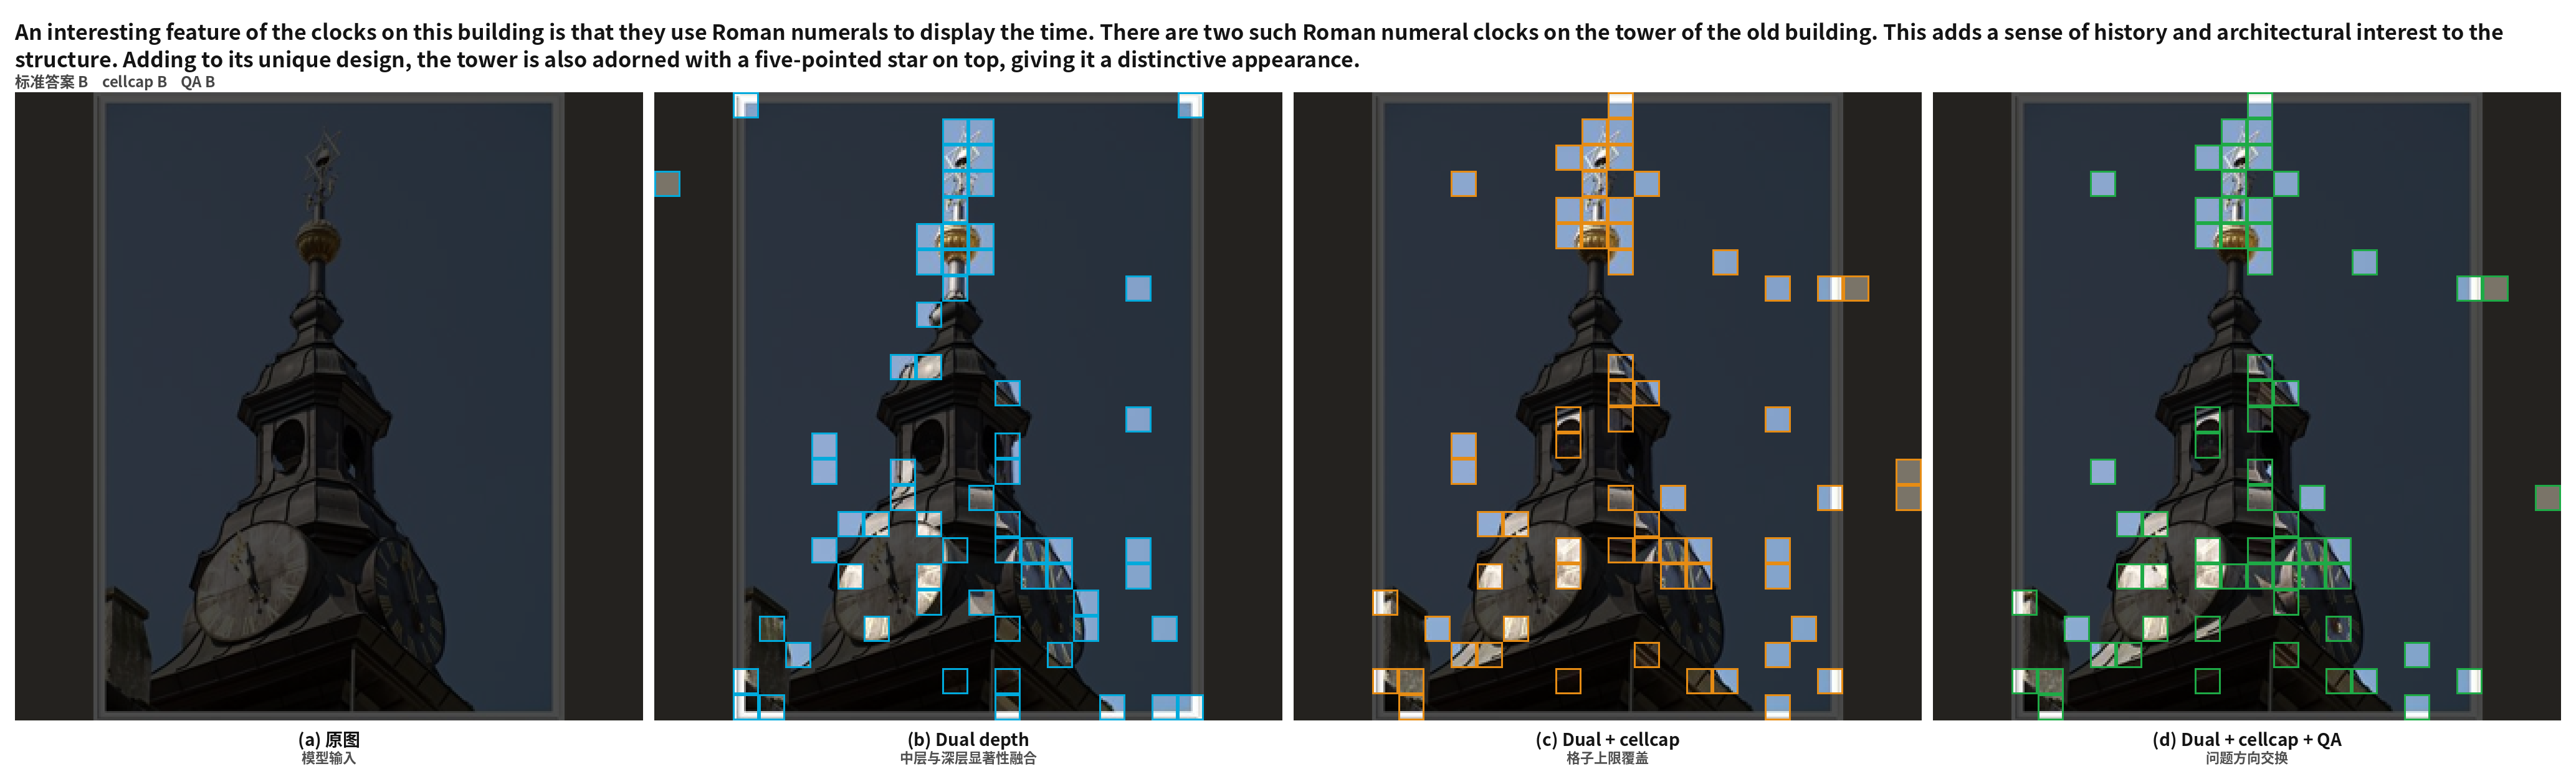
\includegraphics[width=\linewidth]{figures/mmbench_clock.png}
\caption{MMBench 钟楼。金标为 B，格子配额和问题交换都答 B。配额比双深度多亮出外围格子，交换再把一部分亮块收回钟面。}
\label{fig:clock}
\end{figure}

\begin{figure}[h]
\centering
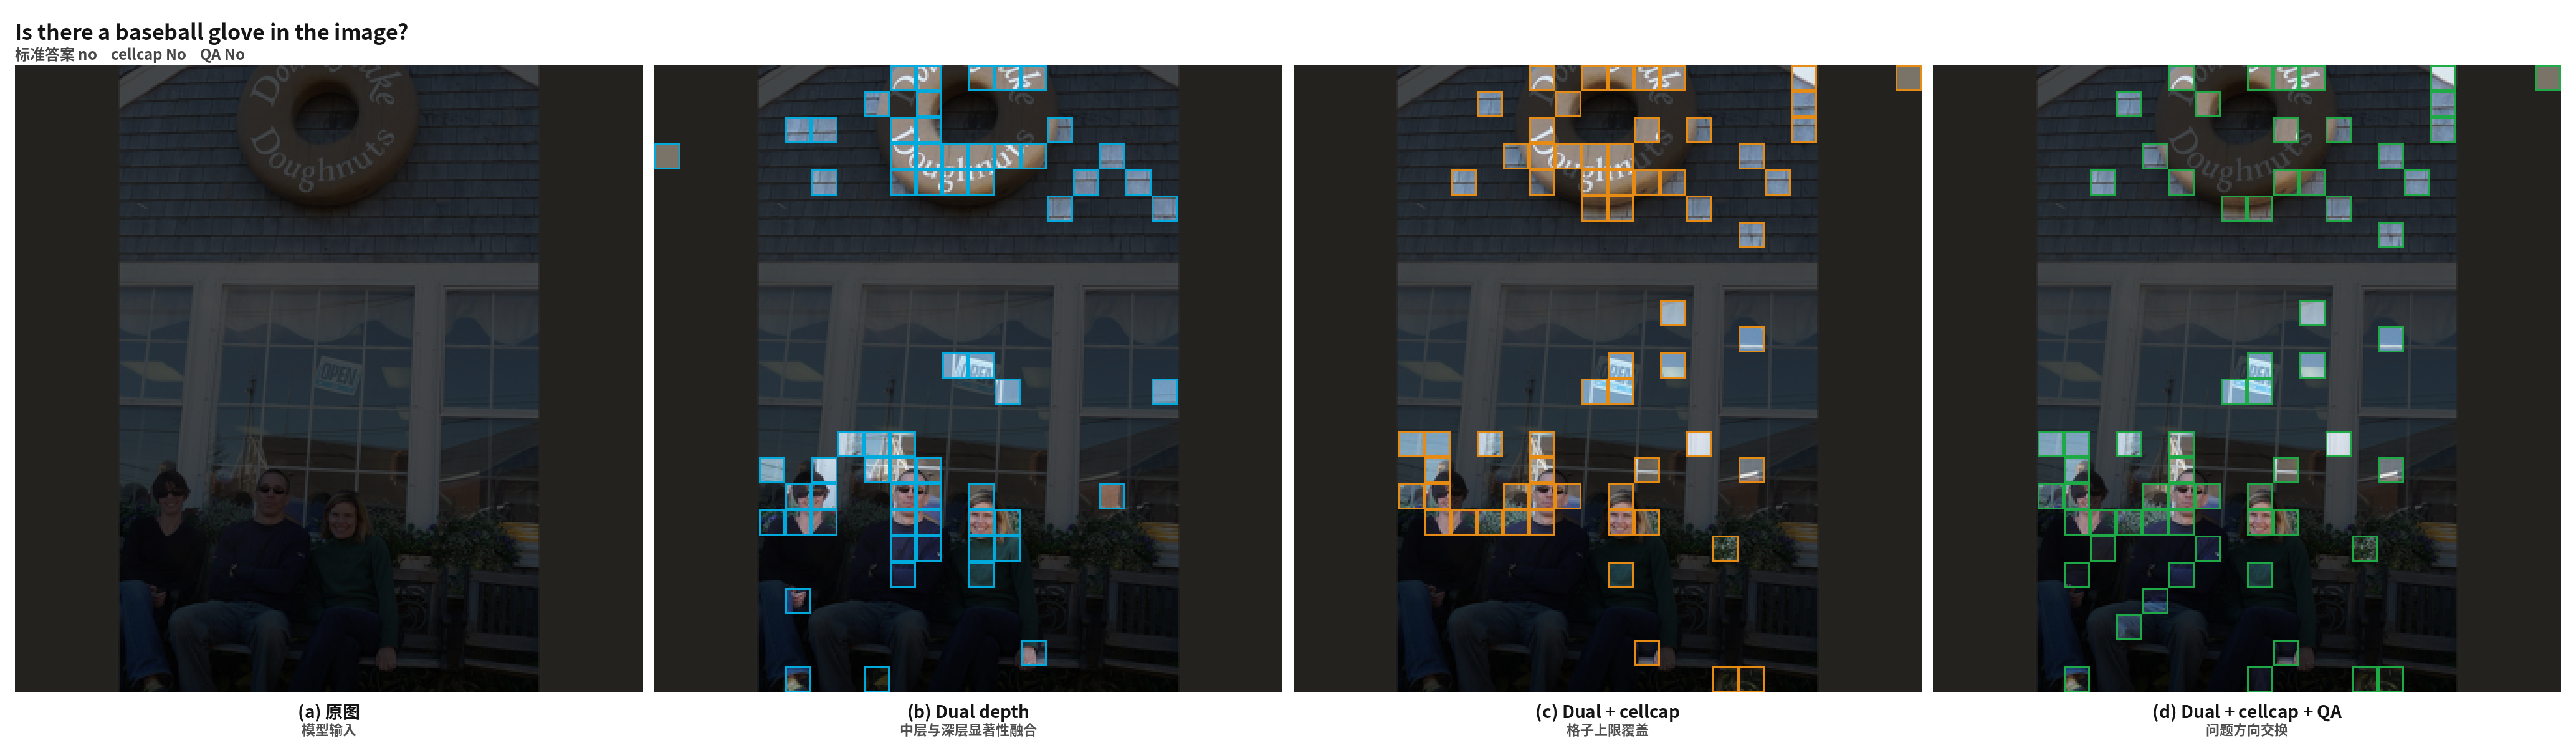
\includegraphics[width=\linewidth]{figures/pope_ring.png}
\caption{POPE：图中是否有棒球手套。金标为 No，两种入口都答 No。交换把一部分亮块从救生圈上的文字移到下方人物。此例只说明位置变化。}
\label{fig:ring}
\end{figure}

式~\eqref{eq:q} 的截断区间和分母里的常数 2 是产生当前分数的实现，换模型时不自动沿用。关系词从查询方向中去掉，仍留在语言模型输入里。标准差过小或内容词为空时不交换。候选池大小、$\lambda_r$、$\lambda_c$、$\gamma$、$\eta$、$\varepsilon$ 和 $\tau$ 的初值同样属于配置。效率测量建议先固定约 200 个图像问题，预热 20 次，再至少重复三轮；GPU 计时在边界同步，报告中位数、均值和 P90。固定长度计时统一生成 32 个 token，并与自然停止的准确率分开保存。
